\documentclass[a4paper]{article}
\usepackage[utf8]{inputenc}
\usepackage[spanish, es-tabla, es-noshorthands]{babel}
\usepackage[table,xcdraw]{xcolor}
\usepackage[a4paper, footnotesep = 1cm, width=20cm, top=2.5cm, height=25cm, textwidth=18cm, textheight=25cm]{geometry}
%\geometry{showframe}

\usepackage{tikz}
\usepackage{amsmath}
\usepackage{amsfonts}
\usepackage{amssymb}
\usepackage{float}
\usepackage{graphicx}
\usepackage{caption}
\usepackage{subcaption}
\usepackage{multicol}
\usepackage{multirow}
\setlength{\doublerulesep}{\arrayrulewidth}
\usepackage{booktabs}
\usepackage{mathrsfs,amsmath}
\usepackage{hyperref}
\hypersetup{
    colorlinks=true,
    linkcolor=blue,
    filecolor=magenta,      
    urlcolor=blue,
    citecolor=blue,    
}

\newcommand{\quotes}[1]{``#1''}
\usepackage{array}
\newcolumntype{C}[1]{>{\centering\let\newline\\\arraybackslash\hspace{0pt}}m{#1}}
\usepackage[american]{circuitikz}
\usetikzlibrary{calc}
\usepackage{fancyhdr}
\usepackage{units} 

\graphicspath{./Imagenes}

\pagestyle{fancy}
\fancyhf{}
\lhead{22.05 ASSD}
\rhead{Mechoulam, Lambertucci, Rodriguez, Londero}
\rfoot{Página \thepage}

\begin{document}

\subsection{Introducción}

Se quiso diseñar y simular el sistema mostrado en la Figura(\ref{fig:sist}). Para esto, se diseño un oscilador que lidie con las señales de control del sistema, un filtro anti-alias y recuperador, el bloque de sample and hold y de la llave analógica. Como primera instancia, se quiso abordar el tema desde un punto teórico, por ende, se deducirán las fórmulas matemáticas para cada nodo del sistema.

\begin{figure}[H]
	\centering
	\includegraphics[width=\textwidth]{ImagenesEjercicio1/sistema.png}
\caption{Esquema del sistema sin señales de control.}
	\label{fig:sist}
\end{figure}

Siendo $X_{in}(t)$ la señal de entrada analógica al sistema, para que esta sea inequívocamente representada por muestras equiespaciadas en el tiempo debe ser el periodo de muestreo menor a la mitad del periodo de la señal de entrada, es decir, sea $f_{in}$ la componente de mayor frecuencia de señal de entrada y $f_s$ la frecuencia de muestreo

\begin{equation}
f_{s} > f_{in}
\end{equation}

Debido a esto, se utiliza un filtro pasabajos para limitar en frecuencia la señal de entrada. Este filtro se denomina filtro anti-alias, dado que al muestrear por debajo del susodicho límite la relación entre la señal muestreada y la señal original no es más unívoca. Estas señales que pueden ser confundidas por la señal de entrada original se denominan aliases.


Ahora que nuestra señal de entrada puede ser inequívocamente representada por un muestreo en tiempo, se procede a obtener la fórmula matemática. Para esto, se deben definir dos formas de muestrear una señal: muestreo natural y muestreo instantáneo. El muestreo natural se realiza con el sistema de la Figura (\ref{fig:sist}) bypasseando el bloque de sample and hold, mientras que el muestreo instantáneo se realiza con el sistema entero.

\begin{figure}[H]
\centering
\begin{subfigure}[b]{.45\linewidth}
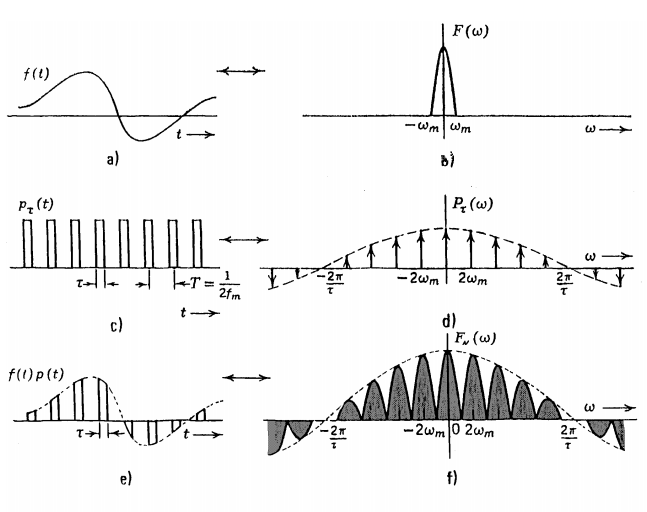
\includegraphics[width=\linewidth]{/ImagenesEjercicio1/Muestreonatural.png}
\caption{Muestreo natural. a-b) Señal original y su espectro c-d) Tren de pulsos y su espectro e-f) Convolución de ambas señales.}
\label{fig:muestreonatural}
\end{subfigure}

\begin{subfigure}[b]{.45\linewidth}
\includegraphics[width=\linewidth]{/ImagenesEjercicio1/Muestreoinstantaneo.png}
\caption{Muestreo natural. a-b) Señal original multiplicada por tren de deltas y su espectro c-d) Pulso y su espectro e-f) Convolución de ambas señales.}
\label{fig:muestreoinstantaneo}
\end{subfigure}
\end{figure}

Finalmente, sea $X_{FAA}$ la señal de entrada limitada en banda, al pasar por el sample and hold la señal multiplicada por un tren de deltas es convolucionada con un pulso obteniendo $X_{SH}$, es decir

\begin{equation}
X_{SH} = \sum_{ahre}^{ayche}
\end{equation}

\subsection{Oscilador}

Para realizar el muestreo y las subsiguientes mediciones se requiere diseñar un oscilador con frecuencia y duty cycle variable. El diseño elegido es el siguiente:

\begin{figure}[H]

	\centering
		\begin{circuitikz}
			\draw
			node[dipchip](555){555}
			
			(555.pin 1) to[short] ++ (-1.3,0)
				to[short] ++ (0, -0.2)
				node[tlground]{}
				
			(555.pin 8) to [short] ++ (1,0)
				to[short] ++ (0, 0.95)
				to[short] ++ (2, 0)
				node[ocirc, label=east:$V_{in}$]{}
			
			(555.pin 7) to [short] ++ (3,0)
				node[ocirc, label=east:$V_{out}$]{}
				++ (-1, 0)
				to[R=$R_1$, *-*] ++ (0, 1.5)
				++ (-1, 0)
				to[short, *-] ++ (-6, 0)
				to[R=$R_2$, -*] ++ (0, -2.06)
				to[R=$R_3$] ++ (0, -2)
				node[ground]{}
				++(0, 2) to[pR=$RP_{freq}$, mirror, name=fpot] ++ (2.757,0)
				(fpot.wiper) to[short] ++ (0,-1.5)
					to[short] ++ (0.8, 0)
					++ (0.55, 0.646)
					to[pR=$RP_{DT}$, mirror] ++ (0, -1.3)
					to[short] ++ (0.75, 0)
					++(-1,0) ++ (0.24, 1.3)
					to[short] ++ (0.75,0)
					to[D=$D_1$] ++ (1, 0) to[short] ++ (0.5,0)
					++(-0.5,-1.3) to[D=$D_2$] ++ (-1,0)
					++(1,0) to[short] ++ (0.5, 0)
					to[short, -*] ++ (0,0.65) to[short] ++ (0,0.65)
					++ (0, -0.65) to[short, -*] ++ (1.75,0)
					to[C=$C_2$] ++ (0,-1.5) node[ground]{}
					++(0,1.5) |- (555.pin 6)
			(555.pin 5) to[short]++(2.5,0)
				to[C=$C_1$] ++ (0, -1) node[ground]{}
			
			(555.pin 4) to[short] ++ (-0.5, 0)
				to[short, -*] ++ (0, 2.615)
			
			(555.pin 2) to[short] ++ (0, 1.115)
				to[short] ++ (2.70, 0)
				to[short, -*] ++ (0, -1.675)		
			
			;
		\end{circuitikz}
	\caption{Oscilador con ajuste de frecuencia y duty cycle independientes.}
	\label{fig:osc}

\end{figure}

Este permite, con los valores tomados mostrados a continuación, variar la frecuencia entre $\approx 9.66kHz$, levemente menor a la frecuencia de corte de nuestro filtro anti-alias, y $25kHz$, logrando traspasar a la frecuencia de Nyquist en un $25\%$. Además, este circuito permite configurar el duty cycle de la señal entre $\approx1\%$ y $\approx99\%$ con máxima frecuencia y entre $\approx5\%$ y $\approx95\%$ con mínima frecuencia. Existe como se puede ver una muy pequeña interacción entre el ajuste de frecuencia y duty cycle, lo que genera que los límites del duty cycle se achiquen al disminuir la frecuencia, pero a fines prácticos se la consideró insignificante dado que los límites mínimos se cumplen.

Los valores tomados se detallan a continuación:

\begin{table}[H]
\centering
\begin{tabular}{cc}
\hline
Componente & Valor \\ \hline
$R_1$ & $2.2 \ k\Omega$ \\
$R_2$ & $10 \ k\Omega$ \\
$R_3$ & $10 \ k\Omega$  \\
$RP_{freq}$ & $4 \ k\Omega$  \\
$RP_{DT}$ & $45 \ k\Omega$  \\
$C_1$ & $10 \ nF$  \\
$C_2$ & $1 \ nF$\\ \hline
\end{tabular}
\caption{Componentes del oscilador.}
\end{table}

Una peculiaridad de esta configuración circuital del 555 es que la salida se encuentra tomada en el pin de descarga del integrado. Esta configuración funciona dado que el pin de descarga y el pin de salida del 555 se encuentran en contra-fase. Esto permite realizar la carga y descarga del capacitor $C_1$ mediante la salida del integrado. Además, las resistencias $R_2$ y $R_3$ aumentan el rango de variabilidad de frecuencias y duty cycle del oscilador. Como el pin de descarga del 555 es de tipo open collector, se debe atar esta salida a la tensión de alimentación mediante una resistencia de pull up, en este caso $R_1$.
Los resultados del oscilador, con una alimentación de $5V$ se muestran a continuación:

\begin{figure}
\centering
\begin{subfigure}[b]{.45\linewidth}
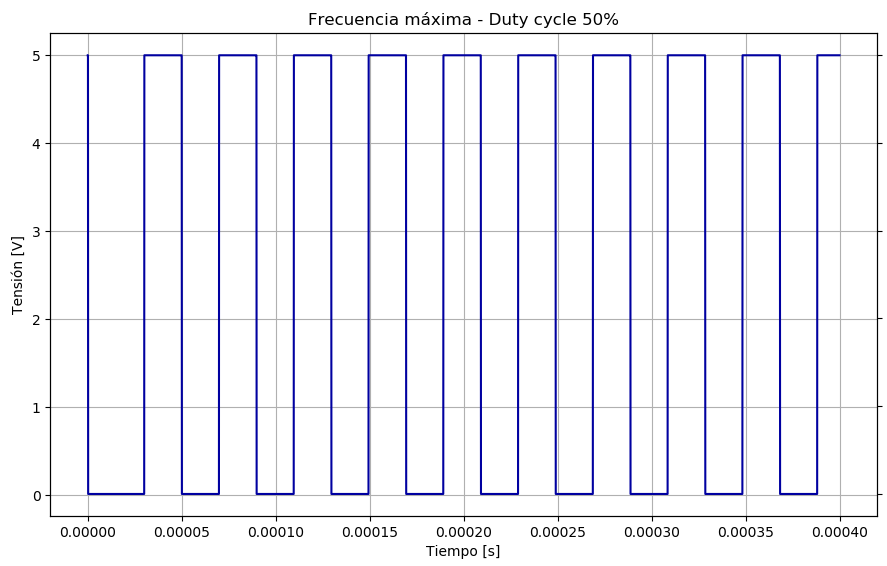
\includegraphics[width=\linewidth]{/ImagenesEjercicio1/DT50FMAX.png}
\caption{Onda simétrica con máxima frecuencia.}
\end{subfigure}
\begin{subfigure}[b]{.45\linewidth}
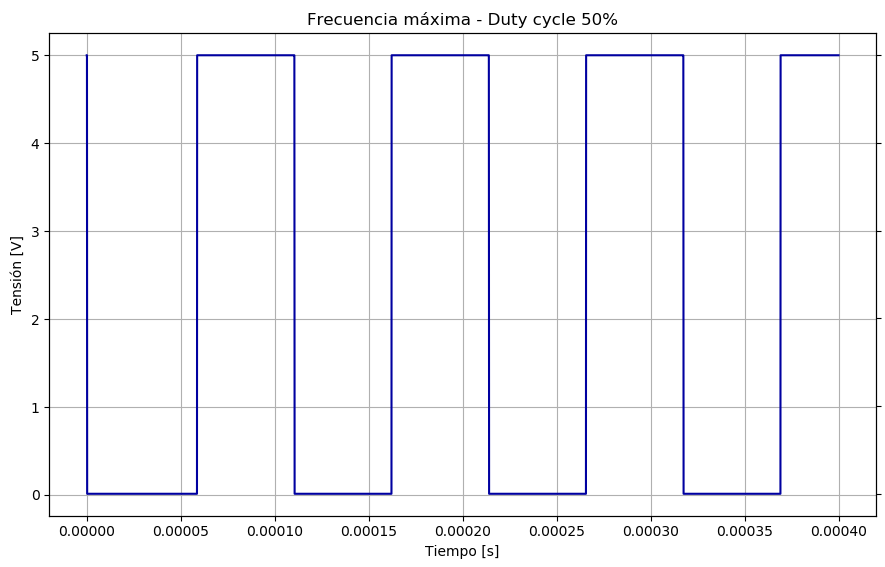
\includegraphics[width=\linewidth]{/ImagenesEjercicio1/DT50FMIN.png}
\caption{Onda simétrica con mínima frecuencia.}
\end{subfigure}

\begin{subfigure}[b]{.45\linewidth}
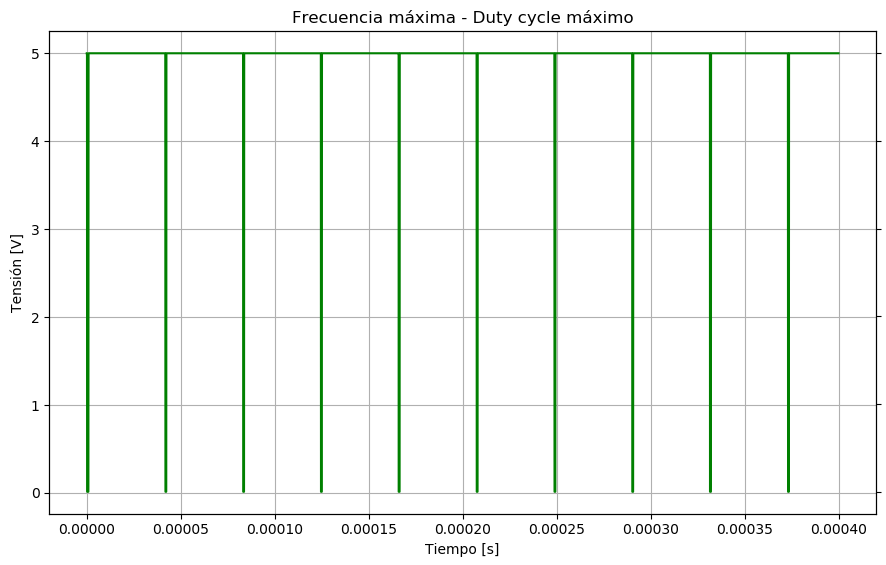
\includegraphics[width=\linewidth]{/ImagenesEjercicio1/DTMAXFMAX.png}
\caption{Máximo duty cycle con máxima frecuencia.}
\end{subfigure}
\begin{subfigure}[b]{.45\linewidth}
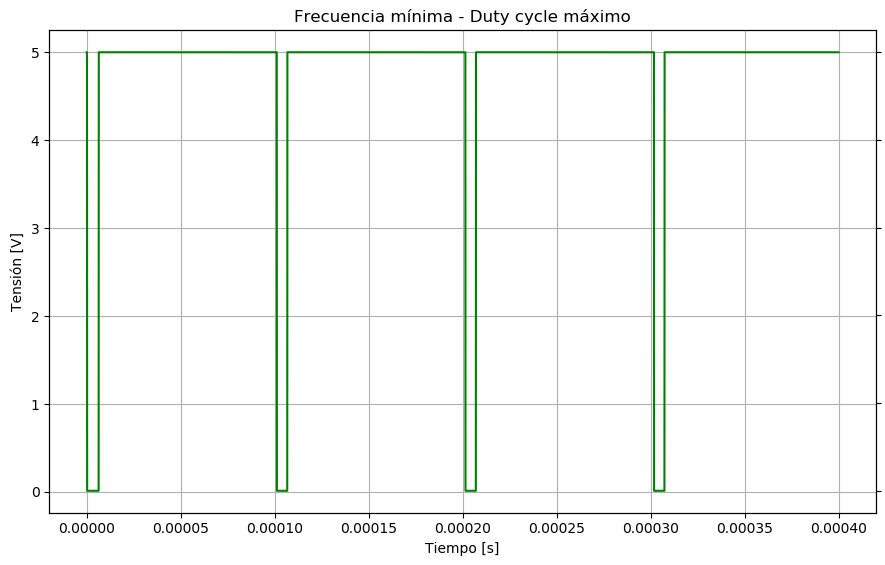
\includegraphics[width=\linewidth]{/ImagenesEjercicio1/DTMAXFMIN.png}
\caption{Máximo duty cycle con mínima frecuencia.}
\end{subfigure}

\begin{subfigure}[b]{.45\linewidth}
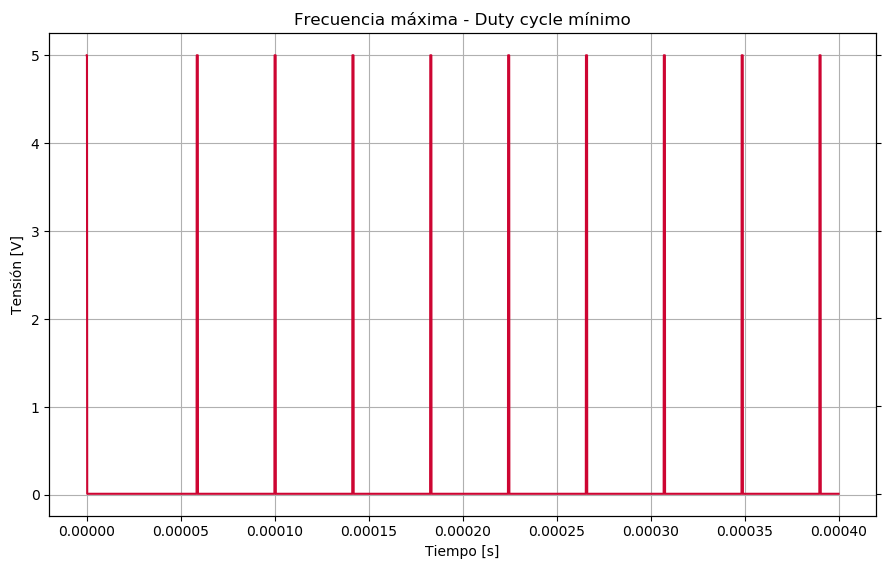
\includegraphics[width=\linewidth]{/ImagenesEjercicio1/DTMINFMAX.png}
\caption{Mínimo duty cycle con máxima frecuencia.}
\end{subfigure}
\begin{subfigure}[b]{.45\linewidth}
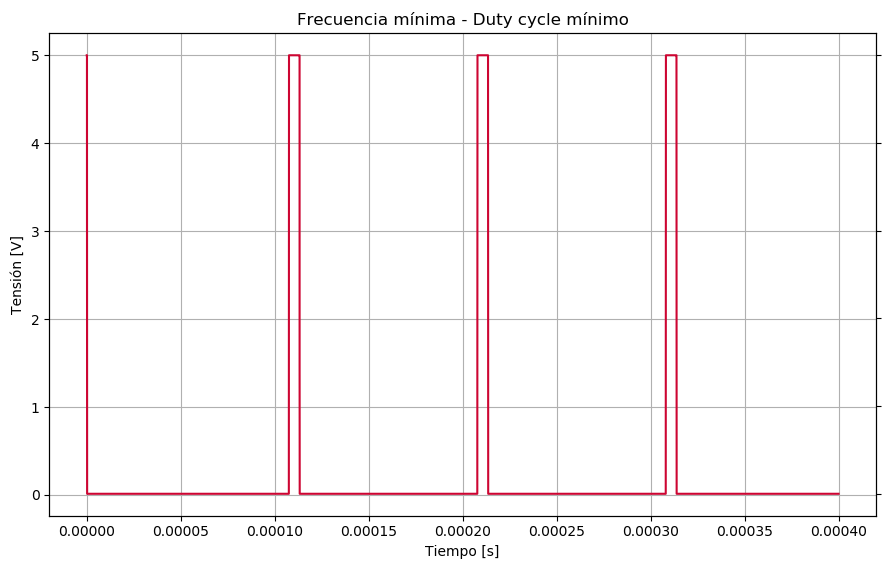
\includegraphics[width=\linewidth]{/ImagenesEjercicio1/DTMINFMIN.png}
\caption{Mínimo duty cycle con máxima frecuencia.}
\end{subfigure}

\end{figure}

\end{document}